\chapter{Hardwarové komponenty}

\section{Sběrnice}

Sběrnice je do jisté míry nervovým systémem celého emulátoru, neboť
nejenom že propojuje hlavní hardwarové komponenty, ale musí se také starat
o jejich paměťovou správu. Díky tomuto faktu sběrnice v emulátoru vytváří všechny komponenty
a řeší jejich vzájemné závislosti.

Jelikož komponenty se mohou navzájem sdílet, bylo nutné zvolit vhodnou strukturu
pro správu jednotlivých objektů. Pro tyto účely jsem se rozhodl použít \textit{shared\_ptr}
ze standardní knihovny \textit{C++}. Nejenom že paměť bude spravována automaticky,
ale lze velice jednoduše vytvořit duplicitní reference na tentýž objekt.

\begin{figure}[hbt]
	\centering
	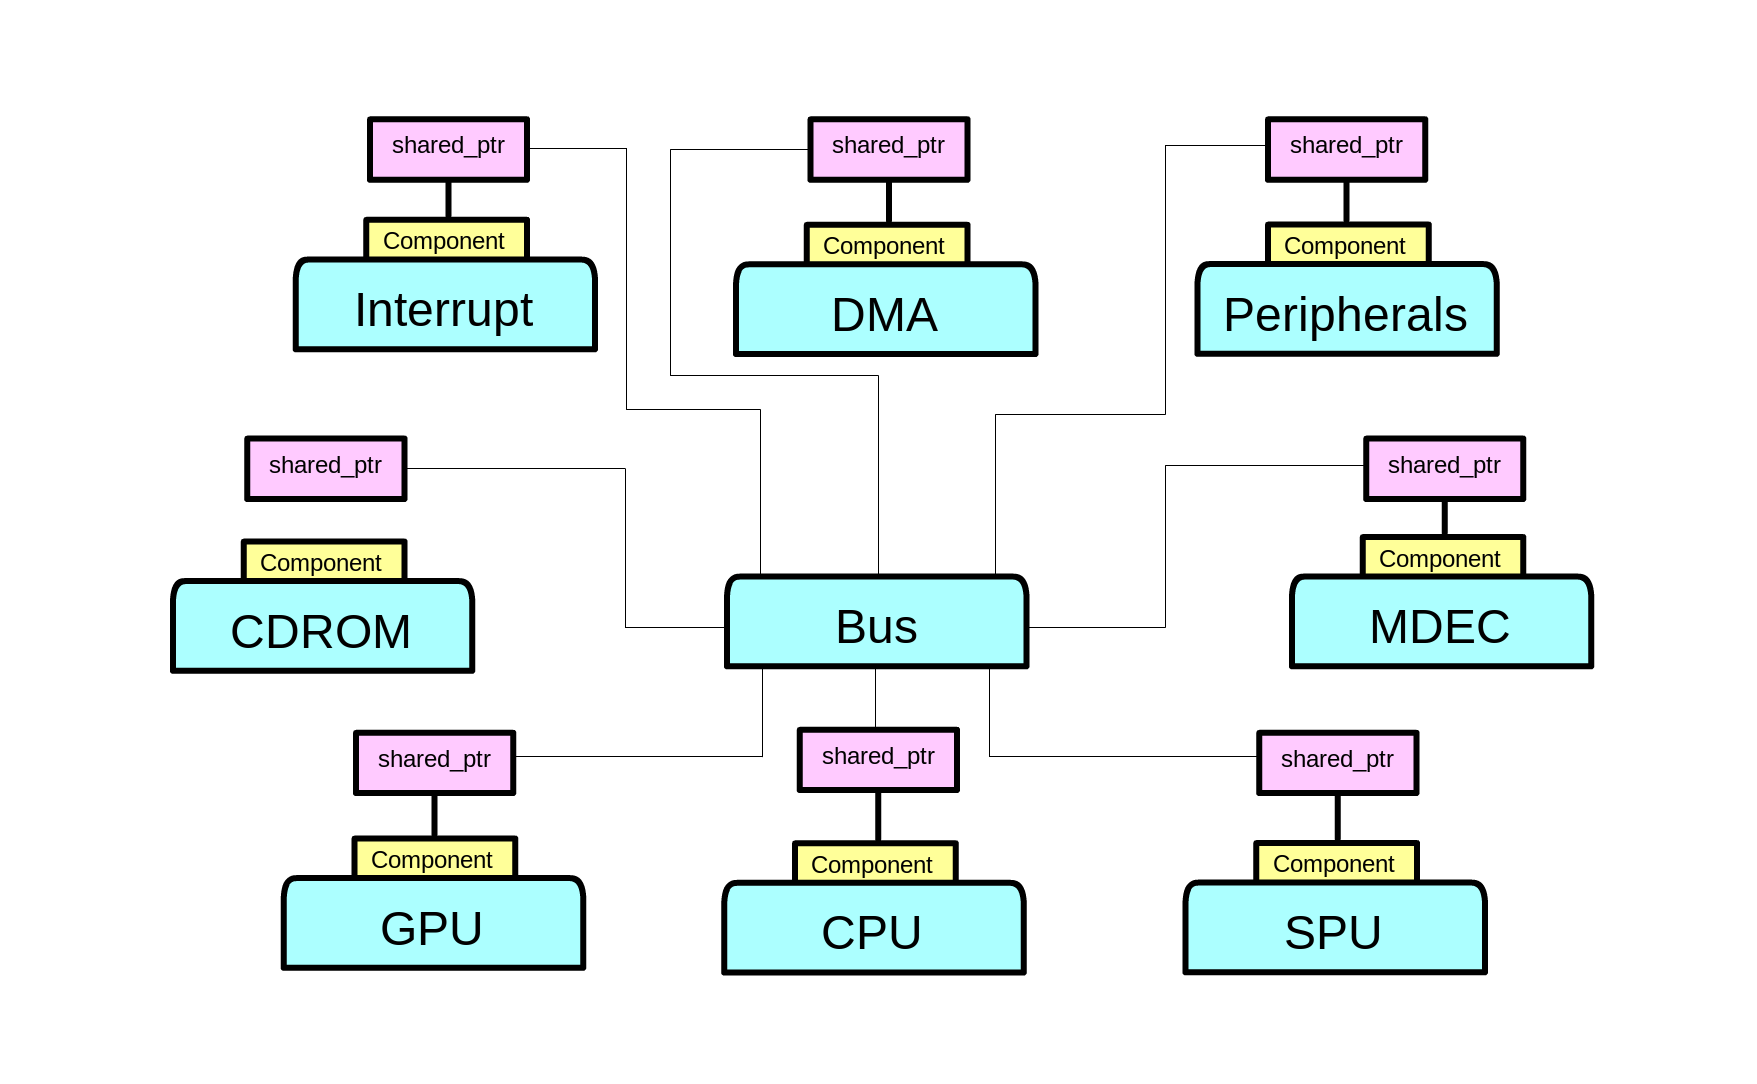
\includegraphics[width=0.8\textwidth]{obrazky-figures/bus-ownage.png}
	\caption{Sběrnice pomocí \textit{shared\_ptr} struktury může vlastnit jednotlivé komponenty, ale také umožňuje tyto komponenty mezi sebou sdílet.}
	\label{bus-ownage}
\end{figure}

Další zodpovědnost sběrnice je správně vysílat čtení a zápisy jednotlivým komponentám.
Všechny tyto paměťové operace závisí na \textit{Memory-mapped I/O}. \textit{Memory-mapped I/O}
mapuje lineární 32-bitový paměťový prostor na segmenty, skrz které může sběrnice ovládat
jednotlivé komponenty.

\begin{table}[htbp]
\caption{Paměťová mapa}
\begin{center}
\begin{tabular}{ |c|c|r| }
 \hline
 \textbf{Název} & \textbf{Lokace} & \textbf{Velikost} \\
 \hline
 RAM & 0x00000000 & 2 MiB \\
 Expansion & 0x1F000000 & 1 MiB \\
 Scratchpad & 0x1F800000 & 1 KiB \\
 Ovladač paměti & 0x1F801000 & 36 B \\
 Periférie & 0x1F801040 & 16 B \\
 Serial & 0x1F801050 & 16 B \\
 Ovladač RAM & 0x1F801060 & 4 B \\
 Ovladač přerušení & 0x1F801070 & 8 B \\
 DMA & 0x1F801080 & 128 B \\
 DotClock Časovač & 0x1F801100 & 16 B \\
 HBlank Časovač & 0x1F801110 & 16 B \\
 SystemClock/8 Časovač & 0x1F801120 & 16 B \\
 CDROM & 0x1F801800 & 4 B \\
 GPU & 0x1F801810 & 8 B \\
 MDEC & 0x1F801820 & 8 B \\
 SPU & 0x1F801C00 & 1 KiB \\
 I/O porty & 0x1F802000 & 8 KiB \\
 BIOS & 0x1FC00000 & 512 KiB \\
 Ovladač cache & 0x1FFE0130 & 4 B \\
 \hline
\end{tabular}
\end{center}
\end{table}

Jelikož sběrnice má 32-bitovou šířku, mohlo by se zdát, že pouze stačí na základě paměťové mapy
vzít danou adresu a rozdistribuovat ji příslušné komponentě. Nicméně sběrnice tohoto systému má
2 zvláštnosti: Správa virtuální paměti a přímý zápis do vyrovnávací paměti instrukcí.

\subsection{Virtuální paměť}

Jak bylo naznačeno, \textit{PlayStation} je do jisté míry zjednodušená verze deskového počítače
a existují určité artefakty, které jsou pozůstatky z plné funkčnosti deskového počítače. Jedním z takovýchto
artefaktů je virtuální paměť. I přesto, že procesor má podporu \textit{Translation Lookaside Bufferu (TLB)},
\textit{PlayStation} jej vůbec nevyužívá a všechny přístupy do paměti jsou skoro absolutní.
Co zůstalo z virtualizace paměti je maskování všech adres, které přijdou na sběrnici a na základě
velikosti zapisovaných či čtených dat, maskování probíhá odlišně.

Nejdříve se u každého přístupu zahodí vrchní 3 bity, pak u půl-slova (16 bitů) se zahodí spodní 1 bit a u slova (32 bitů) se zahodí spodní 2 bity.
Zahození spodních bitů souvisí se zarovnáním do paměti.

\subsection{Vyrovnávací paměť instrukcí}

Druhá zvláštnost, na kterou je třeba myslet při distribuci čtení a zápisu, je vyrovnávací pamět instrukcí
uvnitř \textit{CPU}. Tato vyrovnávací paměť slouží pro ryché získávání instrukcí z hlavní paměti a
teoreticky by nikdy neměla nastat situace, kdy ve vyrovnávací paměti bude něco jiného, než co je
obsaženo v hlavní paměti, ovšem to není u tohoto systému vždy pravda.

\textit{CPU} má speciální stav, který se dá programaticky nastavit, a který takzvaně izoluje vyrovnávací paměť instrukcí.
Pokud \textit{CPU} se nachází v tomto stavu, pak každé čtení za účelem získat instrukci (\textit{fetch} fáze \textit{CPU}) nikdy nebude putovat
do hlavní paměti, ale do této vyrovnávací paměti a \textbf{každý} zápis bude modifikovat vyrovnávací paměť místo hlavní paměti.
\textit{CPU} tedy jinými slovy poskytuje přímý přístup do této paměti.

Pokud toto není správně ošetřeno a simulováno, \textit{PlayStation} nebude schopen nastartovat.

\subsection{Časování}

Každá hardwarová komponenta v reálném čase pracuje paralelně a nezávisle. Situaci také zhoršuje fakt,
že každá komponenta má různou frekvenci hodin.

\begin{itemize}
    \label{Rychlost hodin komponent}
    \item{\textbf{CPU} - 33.868800MHz}
    \item{\textbf{GPU} - 53.222400MHz}
    \item{\textbf{SPU} - 44.100KHz}
    \item{\textbf{DotClock Timer} - 4.980705MHz (Průměr)}
    \item{\textbf{HBlank Timer} - 9923Hz (NTSC), 9943Hz (PAL)}
    \item{\textbf{System Clock/8 Timer} - 4.233600MHz}
\end{itemize}

Tento problém je řešen tak, že v malých kvantech emulátor simuluje každou komponentu sekvenčně a zvlášť,
přičemž množství hodinových cyklů alokované pro danou komponentu reflektuje předchozí tabulku.
To samozřejmě může způsobit časovou dilataci mezi jednotlivými komponentami a může vést k jejich
disinchronizaci. U volby časového kvanta ho nesmíme zvolit příliš malé, protože pak dojde k nesprávnému
zaokrouhlení na základě časovací tabulky a nepřesnost časování bude o to větší, ale zároveň kvantum nesmíme zvolit příliš velké, protože pak
se komponenty nemusí dostat včas ke slovu. Dvě komponenty, pro které je synchronizace nejdůležitější,
jsou \textit{CPU} a \textit{GPU}, přičemž \textit{GPU} je o $11/7$ rychlejší, zvolil jsem tedy časovou konstantu $301$,
protože výsledkem formule $301*11/7=473$ je celé číslo.

\section{CPU}

Pokud sběrnice je nervovým systémem, pak \textit{CPU} je mozkem \textit{PlayStation} systému. Jde
o \textit{MIPS R3000A} 32-bitový \textit{RISC} procesor. Jeho architektura je založená na \textit{MIPS I} redukované instrukční sadě.
\textit{CPU} má celkem 5 stavů, ve kterých se může nacházet a které provádí v nepřetržité smyčce:

\begin{itemize}
    \item{\textbf{Fetch (IF)} fáze - získání následující instrukce z paměti \textit{RAM}.}
    \item{\textbf{Decode (ID)} fáze - získaná instrukce se dekóduje a zjistí se následující operace.}
    \item{\textbf{Execute (EX)} fáze - \textit{CPU} provede dekódovanou instrukci (aritmetickou či logickou operaci).}
    \item{\textbf{Memory Access (MEM)} fáze - pokud získaná instrukce přistupuje do paměti, data jsou pomocí sběrnice přečtena či zapsána.}
    \item{\textbf{Write Back(WB)} fáze - Výsledek instrukce je zapsán do registru.}
\end{itemize}

\subsection{Vnitřní stav \textit{CPU}}

Pro ukládání mezivýsledků a pro obecné účely \textit{CPU} obsahuje celkem \textbf{32} 32-bitových registrů, plus \textbf{2} 32-bitové registry, které
jsou specializované pro práci s násobícími a dělícími instrukcemi. \textit{Nultý} registr je ještě navíc speciální v tom,
že při čtení vždy vrací nulu a jakýkoliv zápis do něj je ignorován.

\subsection{Zpoždění načítání hodnot}

\textit{MIPS R3000A}, jako každý \textit{RISC} procesor, vykazuje zvláštní jev při načítání hodnot do registrů.
Pokud se snažíme načíst hodnotu z paměti \textit{RAM} do procesoru, zpoždění způsobené načítáním hodnoty má za následek
opožděného nastavení registru na přečtenou hodnotu o jeden procesorový takt. 
Toto je způsobeno samotným návrhem \textit{RISC} architektury a je nutné tuto situaci ošetřit. 
V emulátoru je tento fenomén simulován pomocí dvou registrových přihrádek, které figurují jako fronta.
Kdykoliv pak chce \textit{CPU} přečíst hodnotu z paměti \textit{RAM}, místo přímého nastavení registru,
přečtená hodnota spolu s indexem výsledného registru v prvním taktu je vložena do fronty a po druhém taktu se 
zmodifikuje registrové pole.

Je nutné taky pamatovat na situaci, kdy ve frontě je připravená hodnota, ale mezitím přijde jiná instrukce, 
která stejný registr modifikuje. V takovémto případě je nutné frontu vyčistit, aby se výsledný registr špatně
nezmodifikoval.

\subsection{Zpoždění skoku}

Podobně jako opožděné načítání hodnot do registru, design 5 stupňové architektury má za následek ještě jeden problém.
Tento artefakt se objevuje u všech skokových instrukcí a má za následek, že ať se skok provede či neprovede (u podmíněných skoků),
instrukce následující za skokem se vždy provede, protože už je již načtena a zdekódována uvnitř \textit{CPU}. 
Kompilátory té doby s tímto fenoménem počítaly a ve většině případů vyplnily instrukci za skokem prázdnou instrukcí.
Za tímto účelem každý skok v emulátoru je o jeden takt opožděn.

\subsection{Instrukční sada}

Instrukční sada \textit{CPU}, založená na \textit{MIPS I} architektuře, má relativně malý počet instrukcí.
Tato sada obsahuje $40$ bázových instrukcí a $29$ rozšířených instrukcí, což činí dohromady $69$ instrukcí celkem.
Tyto instrukce jsou navrženy tak, aby každá z nich zabrala pokud možno jeden procesorový takt, aby 5-ti úrovňová
linka byla neustále vyplněna. Díky této filozofii, intrukce mají velmi málo zodpovědnosti a jsou ve své podstatě
velmi prostoduché.

Aby se se zamezilo složitému dekódování instrukcí, jak to například je u architektury \textit{x64}, kde každá instrukce
může mít různou délku, \textit{MIPS I} definuje každou instrukci jako 32-bitové dvojslovo, přičemž horních 6 bitů definuje
kódování specifické instrukce. Každou instrukci lze ovšem rozdělit do zhruba tří tříd:

\begin{itemize}
    \item{\textit{opkód} (6 bitů), \textit{zdrojový registr} (5 bitů), \textit{cílový registr} (5 bitů), \textit{výsledný registr} (5 bitů), \textit{shift hodnota} (5 bitů), \textit{kód funkce} (6 bitů)}
    \item{\textit{opkód} (6 bitů), \textit{zdrojový registr} (5 bitů), \textit{cílový registr} (5 bitů), \textit{bezprostřední hodnota} (16 bitů)}
    \item{\textit{opkód} (6 bitů), \textit{cíl skoku} (24 bitů)}
\end{itemize}


\begin{figure}[hbt]
	\centering
	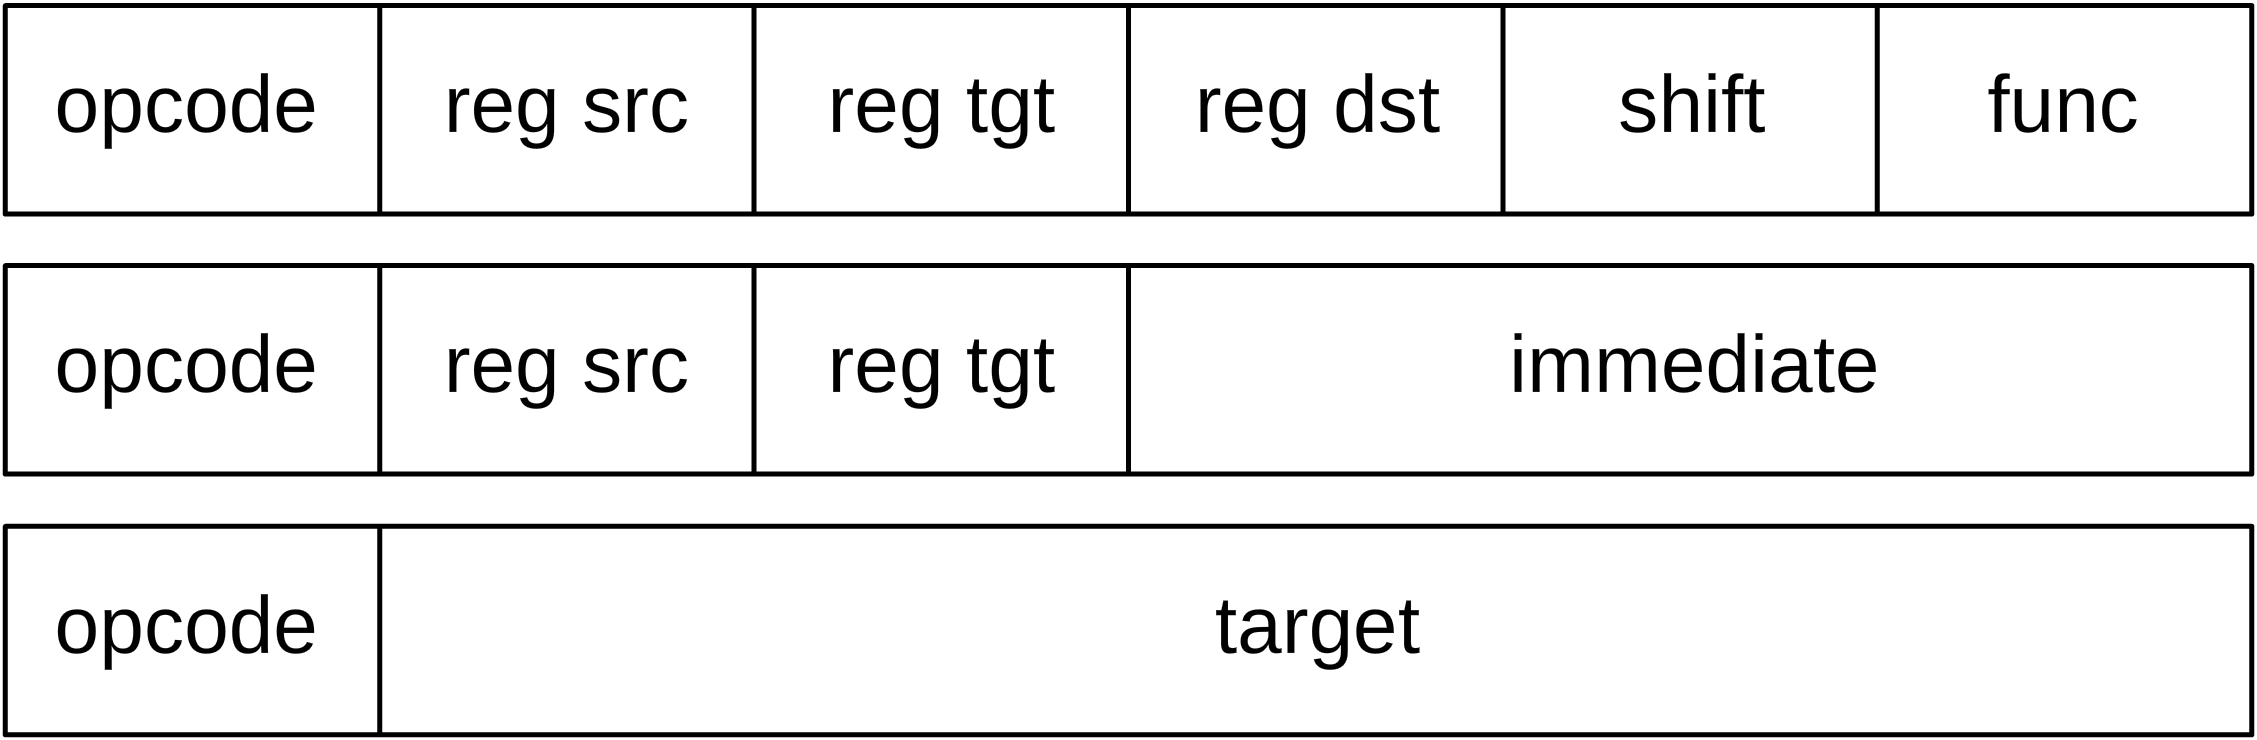
\includegraphics[width=0.8\textwidth]{obrazky-figures/instruction.png}
	\caption{\textit{MIPS} má celkem 3 způsoby, jak zakódovat instrukci do 32 bitů.}
	\label{instruction}
\end{figure}

\subsection{Koprocesory}

\textit{MIPS R3000A} ve své instruční sadě má podporu pro celkem 4 různé koprocesory, ovšem \textit{PlayStation} využívá
pouze 2 z nich. Koprocesorové instrukce jsou versatilní a lze za ně substituovat jakýkoliv čip, až na koprocesor 1, který
je dedikovaný pro práci s čísly s plovoucí desetinou čárkou.

\textit{PlayStation} \textbf{koprocesor 0} využívá pro správu výjimek a přerušení. Koprocesor obsahuje nejenom typ výjimky či kdo
způsobil přerušení, ale také obsahuje logiku pro zpracování výjimky, kde procesoru se uloží současný stav a jeho kontrolní tok je převeden
na rutinu, která se stará o obsluhu výjimky.

\textbf{Koprocesor 2} pak zpřístupňuje komponentu \textit{Geometry Transformation Engine (GTE)}, což je hardware dedikovaný
pro rychlou práci s lineární algebrou. Tento koprocesor má 2 základní datová primitiva, se kterými umí pracovat jsou 3D vektory (16/32-bitový atom) a 3x3 maticemi (16/32-bitový atom).
Vektory se mohou dále interpretovat jako body v prostoru, či jako barva a pro každý typ má \textit{GTE} dedikované příkazy.
Funkcionalita \textit{GTE} je velmi versatilní. Můžeme v něm najít rychlé násobení matice s vektorem, normalizace barev či vektoru, či dokonce interpolace.
Tento koprocesor je bezpochyby velice důležitý pro rychlé zpracování geometrie ve hře a rychlého vykreslení 3D scény.

\section{GPU}

Grafická jednotka systému je speciálně nadesignovaný čip pro hardwarovou podporu rasterizace geometrických primitiv.
\textit{GPU} pracuje na frekvenci 53.222400MHz a tedy je o $11/7$ rychlejší než frekvence \textit{CPU}. Všechna práce s \textit{GPU} probíhá přes
4 registry:

\begin{itemize}
    \item{\textbf{GP0} (pouze zápis) - registr pro zasílání rasterizačních příkazů a zasílání geometrických dat. Různé grafické příkazy mohou mít různou délku.}
    \item{\textbf{GP1} (pouze zápis) - registr pro modifikaci stavu \textit{GPU} (například: reset, rasterizovací okno či potvrzení přerušení).}
    \item{\textbf{GPUREAD} (pouze čtení) - registr pro čtení \textit{VRAM} paměti nebo pro čtení speciálních registrů.}
    \item{\textbf{GPUSTAT} (pouze čtení) - registr pro akumulaci a čtení celkového stavu \textit{GPU}.}
\end{itemize}

\subsection{VRAM}

\textit{GPU} má také svoji vlastní paměť \textit{Video RAM (VRAM)}. Paměť je rozdělena na 512 řádků o 1024 16-bitových slovech.
Celkem tedy paměť \textit{VRAM} má kapacitu $1024*512*2=1'048'576B=1MB$. \textit{VRAM} paměť slouží pouze pro ukládání textur, palety pro
indexované textury a výsledný \textit{framebuffer}. Jakákoliv data o kreslených primitivech (pozice vrcholů či texturovacích koordinátů)
musí být zaslána přes \textbf{GP0} registr. I přesto, že \textit{GPU} má různé módy týkající se barevné hloubky (24 bitů a 15 bitů).
Výsledný framebuffer musí mít formát 15 bitové barvy.

\subsection{Geometrická primitiva}

\textit{GPU} dokáže vykreslit 3 geometrická primitiva:

\begin{itemize}
    \item{Osově zarovnaný obdélník}
    \item{Čára/Polyčára}
    \item{Trojúhelník/Čtyřúhelník}
\end{itemize}

Všechna tato primitiva lze kreslit pomocí \textbf{GP0} registru, přičemž je nutné zapsat správný počet argumentů do tohoto registru.
Počet argumentů daného primitiva závisí především na různých vlastnostech daného primitiva. Ačkoliv ne všechny primitiva mohou mít
všechny vlastnosti, \textit{GPU} dokáže rasterizovat jednotlivá primitiva různými způsoby.

\begin{itemize}
    \item{\textbf{texturovací koordináty} - primitivum má k sobě přiřazenou texturu a každý vrchol má asociované texturovací koordináty}
    \item{\textbf{průhlednost} - na základě předchozího obsahu ve \textit{VRAM} paměti, \textit{GPU} dokáže mixovat barvy ve čtyřech různých módech:
        \begin{itemize}
            \item{\textit{half-each} - $výsledek = \frac{pozadí + zdroj}{2}$}
            \item{\textit{additive} - $výsledek = pozadí + zdroj$}
            \item{\textit{subtracitve} - $výsledek = pozadí - zdroj$}
            \item{\textit{additive/4} - $výsledek = pozadí + \frac{source}{4}$}
        \end{itemize}
    }
    \item{\textbf{Gouraudovo stínování} - tento atribut je trochu zavádějící, neboť gouraudovo stínování souvisí spíše s výpočtem osvětlení. V tomto případě ovšem jde pouze zapnutí interpolace atributů mezi vrcholy primitiva.}
\end{itemize}

\subsection{Barvy}

Jak bylo zmíněno, \textit{GPU} dokáže pracovat s 24-bitovými barvami, které obsahují 3 základní barevné komponenty (červená, zelená a modrá) a
každému z těchto komponent je alokováno 8 bitů a potom dokáže pracovat s 15-bitovými barvami, kde každé komponentě je
přiřazeno pouze bitů 5. 

Ovšem paměť \textit{VRAM} je rozdělena do 16-bitových slov. Je tedy nutné tyto barevné formáty správě mapovat do výsledné 16-bitové barvy.
15-bitová barva se pouze zkopíruje do paměti \textit{VRAM}, přičemž 24-bitová barva je za pomocí techniky \textit{dithering} rozdistribuována
do kreslícího okolí. Paměť \textit{VRAM} v každém pixelu také ukládá extra 1 bit, který figuruje jako kreslící maska. Pokud je nejvyšší bit
v 16-bitové barvě nastaven na 1, pak tento pixel bude ignorován a nic se do něj nevykreslí.

\subsection{Rasterizace primitiv}

U každého ze 3 geometrických primitiv, které \textit{GPU} dokáže vykreslit je nutno zvolit správný algoritmus pro jeho rasterizaci.

U rasterizace osově zarovnaného obdélníku stačí zjistit maximum a minimum ve 2D prostoru tento omezený prostor může být vyplněn.

Rasterizace čáry vyžaduje sofistikovanější přístup, a to \textbf{Digital Differential Analyzer (DDA) algoritmus}, který na základě výpočtu
sklonu čáry, dokáže vyplnit fragmenty mezi dvěma body ve 2D prostoru.

Trojúhelníková rasterizace se řadí mezi vyplňovací rasterizační algoritmy. Pro jeho implementaci jsem zvolil efektivní \textbf{Pinedův algoritmus}.
Jeho podstata závisí na rozdělení jednotlivých hran trojúhelníku na poloroviny a u každého fragmentu zjišťovat jeho polohu, v závislosti na
všech polorovinách daného trojúhelníku.

\subsection{Zvýšení rozlišení}

Zvýšení rozlišení se týká právě \textit{GPU} a rasterizací jednotlivých primitiv. \textit{GPU} ve svém interním stavu
ukládá mimo jiné meze \textit{framebufferu}. Tyto meze pak figurují u rasterizace, kde jakýkoliv pokus kreslit mimo tyto meze
bude ignorován a zároveň tyto meze určují odkud z \textit{VRAM} paměti se budou brát data pro zasílání do \textit{CRT} monitoru.

Pro tyto účely bude nutné spravovat zvláštní \textit{framebuffer}, který podle nastavení bude mít násobek velikosti
současného reálného \textit{framebufferu} uvnitř \textit{GPU}. U každé modifikace mezí reálného \textit{framebufferu} je
nutné zvlášní \textit{framebuffer} zničit a znovu spočítat jeho velikost.

Rasterizace primitiv pak je nutné zachytit a správně přepočítat jejich pozice a upravit jejich omezující vlastnosti.
Největší potíž ovšem bujede u adresace textur a jejich palet. Při každém zápisu textury a indexu barvy je nutné koordináty
přemapovat do zvláštního \textit{framebufferu}.

\section{DMA}

Jelikož \textit{CPU} má hodinovou rychlost 33.8688MHz, jakýkoliv přenost dat je nesmírně pomalý. Tento fakt je pouze amplifikován v situaci
kdy program chce přenést data z paměti \textit{RAM} do jiné hardwarové komponenty. Pokud bychom měli jednoduchou smyčku pro kopírování
dat s prokládanou inkrementací indexu do paměti (abychom vyplnily zpoždění čtení z paměti \textit{RAM}):

TODO
% LW [r1] [r2]      // Load 32-bit value into r1 from address r2
% ADDIU [r2] [r2] 4 // Increment r1 by 4 to move to the next 32-bit value
% SW [r2-4] [r1]    // Store 32-bit value back to ram to address r2

To teoreticky znamená, že rychlost přenosu je $TODO/3=TODO$. Kvůli tomuto neduhu \textit{PlayStation} obsahuje komponentu \textit{Direct Memory Access (DMA)},
která slouží čistě pro velmi rychlý přenos dat mezi pamětí \textit{RAM} a hardwarovými komponentami. \textit{DMA} má celkem 7 různých kanálů,
přičemž každý kanál specifikuje komunikující komponenty. 

\begin{itemize}
    \item{\textbf{0 - MDECIN} - Z \textit{RAM} do \textit{MDEC} vstupu}
    \item{\textbf{1 - MDECOUT} - Z \textit{MDEC} výstupu do \textit{RAM}}
    \item{\textbf{2 - GPU} - Mezi \textit{RAM} a \textit{GPU}}
    \item{\textbf{3 - CDROM} - Z \textit{CD-ROM} do \textit{RAM}}
    \item{\textbf{4 - SPU} - Mezi \textit{RAM} a \textit{SPU}}
    \item{\textbf{5 - PIO} - Mezi \textit{RAM} a \textit{Expansion Port}}
    \item{\textbf{6 - OTC} - Mezi \textit{RAM} a \textit{GPU Ordering Table}}
\end{itemize}

\textit{DMA} také poskytuje celkem 3 různé módy přenosu:

\begin{itemize}
    \item{\textbf{Word Copy} - Jde o rychlý přenos lineární sekvence 32-bitových hodnot. Maximálně se může přenést až 65536 32-bitových hodnot.}
    \item{\textbf{Block Copy} - Přenáší se bloky o uživatelem definované délce. Provedení přenosu také závisí na připravenosti komponenty.}
    \item{\textbf{Linked List Copy} - Přenášená data se dělí na hlavičku a tělo. Hlavička obsahuje délku těla a adresu další hlavičky. Celá datová struktura je pak řetězec hlaviček a těl.}
\end{itemize}

Každý mód přenosu poskytuje velmi rychlé přenosy, protože \textit{DMA} využívá \textit{DRAM Hyper Page} mód,
což umožňuje \textit{DMA} přistupovat k \textit{DRAM} řádkům v jednom procesorovém cyklu. Tento přístup sice
má minimální režii, která způsobí že pro každých 17 cyklů se přečte 16 32-bitových slov.

Při \textit{DMA} přenosu, \textit{CPU} má přísná pravidla ohledně přístupu do paměti. Pokud probíhá přenos,
\textit{CPU} může přistupovat k vyrovnávacím pamětem a ke svým dvěma koprocesorům. Jakmile se \textit{CPU}
pokusí přistoupit do paměti, je jeho chod pozastaven, dokud \textit{DMA} přenos není dokončen.

Díky tomuto faktu lze v emulátoru jakoukoliv \textit{DMA} synchronizaci obejít tím, že celý přenos se provede najednou
a \textit{CPU} je pozastaveno. Výjimkou je \textit{MDEC}, kde tato komponenta indikuje připravenost přenosu dat.

\section{Ovladač přerušení/výjimek}

Aby \textit{CPU} mělo přehled o různých událostech, jako je například dokončení \textit{DMA} přenosu, \textit{PlayStation}
má 2 úzce svázané hardwarové komponenty: \textit{Ovladač přerušení} a \textit{Ovladač výjimek}. \textit{Ovladač přerušení}
je propoje v podstatě se všemi ostatními komponentami, od kterých je schopen přijímat požadavky na přerušení. Tento
čip také obsahuje stavový registr, u kterého se dá zjistit kdo přerušení způsobil.

To ale není dost proto aby byl chod procesoru přerušen. \textit{Ovladač přerušení} je napojen na \textit{koprocesor 0 CPU},
tedy \textit{Ovladače výjimek}, přičemž přerušení je pouze zvláštní typ výjimky.

TODO: exception and interrupt types

\textit{BIOS} potom má předem definované vektory adres, na základě kterých se rozhoduje kam předelegovat řízení procesoru
a následné zpracování výjimky.

\section{Časovače}

\textit{PlayStation} má 3 různé druhy zdrojů hodin, plus jeden hodinový zdroj pro \textit{CPU}. Jelikož
se tyto 3 hardwarové složky příliš nelyší, využil jsem \textit{STL} knihovnu \textit{C++} pro instanciaci
každého ze tří zdrojů. 

\textit{První} zdroj se jmenuje \textbf{Dot Clock}. Tento zdroj souvisí s renderovacím módem \textit{GPU}
komponenty. \textit{Dot} v tomto kontextu reprezentuje jeden vykreslený fragment (tedy ne pixel na obrazovce) a
tento zdroj tedy počítá počet vykreslených fragmentů, přičemž rychlost závisí na vertikálním rozlišení \textit{GPU}.

\textit{Druhý} zdroj také souvísí s \textit{GPU} a jeho jméno je \textbf{Horizontal Blank Clock}. Pokaždé, když \textit{GPU}
dokončí kreslení jednoho řádku \textit{Framebufferu}, tento zdroj je inkrementován o jedničku. Rychlost závisí na
regionu konzole a verze \textit{BIOSu} (\textit{NTSC}/\textit{PAL}).

\textit{Třetí} zdroj je pak \textbf{System Clock}, který reflektuje zdroj hodin \textit{CPU}, ovšem je zpomalen:
$SystemClock=\frac{CPUClock}{8}$.

Každý z těchto časovačů má také schopnost vyvolat přerušení, pokud se dosáhne určité hodnoty. Všechny tyto časovače
kromě svých specifických zdrojů, mají také zdroj hodin \textit{CPU} a jsou schopné svůj zdroj měnit.

\section{MDEC}

Tento hardwarový čip je jedním z hlavních komponent, která učinila \textit{PlayStation} velmi populární konzoli.
Jelikož se \textit{Sony} rozhodlo použít \textit{CD} jako hlavní úložiště pro hry, každá hra měl na tu dobu 
velký prostor. V porovnání se svým protivníkem \textit{Nintendem 64}, které mělo možnost úkládat maximálně \textit{64 MB},
\textit{PlayStation} disponoval až \textit{600 MB}, přičemž hra mohla mít i vícero disků, a hráč mohl jednotlivé
disky měnit na základě postupu ve hře.

Takový prostor bylo třeba využít a \textit{Sony} se rozhodl pro video. \textit{MDEC} je čip speciálně dedikovaný
pro dekódování speciálního formátu videa. Hlavní myšlenkou tohoto formátu byl \textit{JPEG}. \textit{JPEG} používá
několik kopresních technik, které efektivně zkombinuje dohromady. Obrázek je rozdělen na \textit{Makrobloky}, 8x8 nebo 16x16
bloky pixelů. Tyto bloky jsou poté převedeny do \textit{YCbCr} barevného formátu a \textit{CbCr} složky se o polovinu
zmenší. Toto si můžeme dovolit, protože lidské oko je citlivější na intenzitu světla, než na samotnou diferenci barev.
Poté se provede \textit{Discrete Cosine Transform (DCT)} frekvenční analýza a pomocí kvantizační tabulky se odstraní přebytečné frekvence. 
Výsledný makroblok přeskládán \textit{Zig Zag} vzorem je a zakódován pomocí \textit{Run-Length} kódování.
\textit{JPEG} pak využije \textit{Huffmanova} kódování pro vytvoření výsledného toku dat.
Dekódování probíhá velice podobně, ale naopak. 

Formát snímku videa v \textit{PlayStationu} je velice podobný \textit{JPEGu}, až
na ten rozdíl, že \textit{PlayStation} nevyužívá \textit{Huffmanova} kódování.

\begin{figure}[hbt]
	\centering
	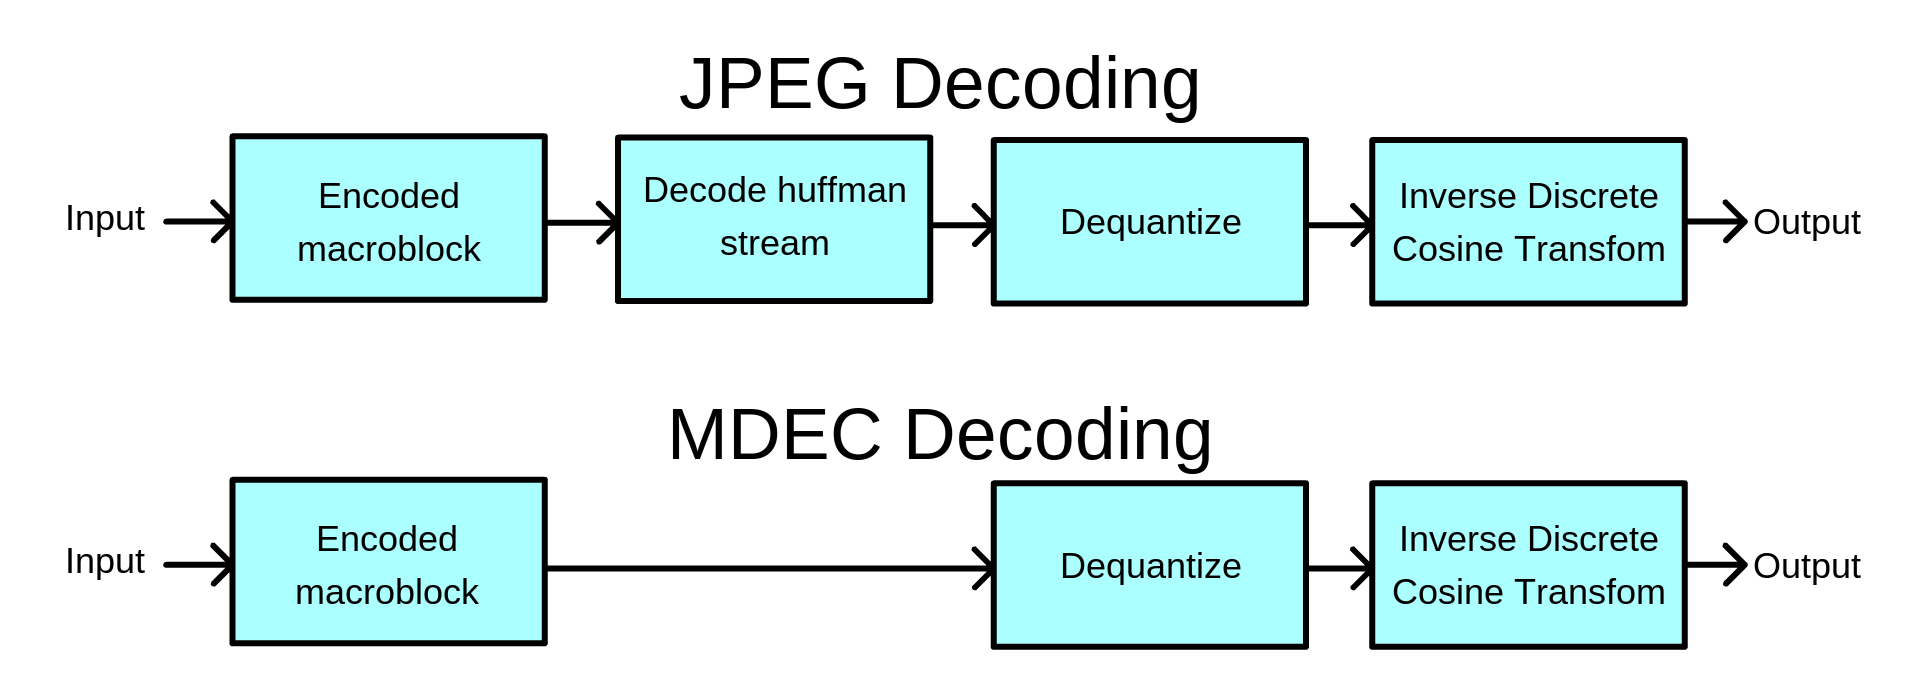
\includegraphics[width=0.8\textwidth]{obrazky-figures/mdec-decoding.png}
	\caption{\textit{MDEC} má velmi podobnou strukturu jako \textit{JPEG} až na vynechaný krok Huffmanova dekódování.}
	\label{mdec-decoding}
\end{figure}

Při přesunu dat, \textit{MDEC} má speciální příznak pomocí kterého indikuje stav dekódování (připravenost vstupu a výstupu).

\section{CD-ROM mechanika}

\textit{Sony} se rozhodlo použít pro herní úložiště použít \textit{Compact Disc Extended Architecture (CD-XA)} a ISO 9660 standard.
Ačkoliv \textit{BIOS} se stará o analýzu ISO 9660 soborového systému, \textit{PlayStation} obsahuje speciální \textit{CD-ROM} mechaniku
pro čtení \textit{CD}. 

\textit{CPU} může komunikovat s \textit{CD-ROM} mechanikou jednak přes registry a příkazy, ale \textit{CD-ROM} má také 3 datové fronty,
pomocí nichž se přenášejí data a dotazy na přerušení. Interně \textit{CD-ROM} má celkem \textit{37} příkazů, pomocí kterých
lze manipulovat se čtecím motorem.

Pro správný přístup k \textit{CD} je nutné správně toto médium adresovat. Jelikož \textit{CD-ROM} je spíše chápáno jako
uložiště pro audio či video média, disk je adresován pomocí stop, přičemž každá stopa se dá reprezentovat indexem,
nebo formátem \textit{minuty(MM):sekundy(SS):zlomky(FF)}. Každý disk má maximálně \textit{74} minut, přičemž v každé minutě
je \textit{60} sekund a každá sekunda obsahuje \textit{75} zlomků. S touto znalostí se pak tento 
formát dá převést na \textit{Logical Block Addresssing (LBA)}, tedy schopnost adresovat \textit{CD} jako lineární paměť bytů.

Hry také měli možnost být prodávány ne na jednom, ale na několika discích. \textit{CD-ROM} má pak schopnost výměny disku
bez resetu konzole. Pomocí vypnutí motoru lze \textit{CD-ROM} mechaniku pozastavit, otevřít poklop, disk vyměnit
a program po uzavření poklopu může bezproblémově pokračovat.

\section{Periférie}

Ačkoliv samotná konzole má vnitřně několik typů periférií, jako jsou I/O a debugovací porty, veřejně dostupná verze konzole má celkem 4 porty,
se kterými běžný uživatel může interagovat. 2 z těchto portů slouží na vsunutí \textit{MemoryCard}, což figurovalo jako malé uložiště, které sloužilo
pro uložení postupu ve hrách. Zbylé 2 porty pak fungovali jako vstupy pro herní ovladače, kde existovali celkem 3 podporované typy: \textit{Digital}, \textit{Analog} a \textit{Mouse}.
Nicméně drtivá většina celé \textit{PlayStation} knihovny pouze používala \textit{Digital} verzi ovladače.

Hry pak mohli individuálně z těchto portů číst a umožnili tak uživateli s konzolí pracovat.
Všechna komunikace mezi \textit{CPU} a perifériemi probíhá pomocí \textit{Serial I/O (SIO)}.













